\documentclass{article}
\author{Max Springenberg, 177792}
\title{
    DAP2 UB12\\
    Anja Rey, Gr.23 , Briefkasten 22
}
\date{}
\usepackage{amsmath}
\usepackage{amssymb}
\usepackage{stmaryrd}
\usepackage{graphicx}
%graphs
\usepackage{tikz}
\usepackage{tikz,fullpage}
\usetikzlibrary{arrows,%
                petri,%
                topaths}%
\usepackage{tkz-berge}
\usepackage[position=top]{subfig}
% sheet number
\setcounter{section}{13}
% \Theta \Omega \omega
\newcommand{\tab}{\null \qquad}
\newcommand{\lA}{$\leftarrow$}
\newcommand{\ue}{$\infty$}

\begin{document}
\maketitle

\newpage
\subsection{Negative Kanten und Bellman-Ford}
\subsubsection \
Gegeben sei der Graph $G$:\\
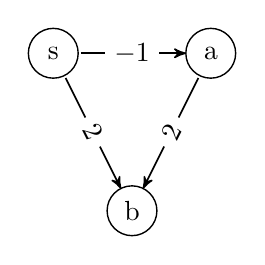
\begin{tikzpicture}[scale = 1.0, transform shape]
    \Vertex[x=0,y=2]{s}
    \Vertex[x=2,y=2]{a}
    \Vertex[x=1,y=0]{b}
    \tikzstyle{LabelStyle}=[fill=white,sloped]
    \tikzstyle{EdgeStyle}=[post]
    \Edge[label=$-1$](s)(a)
    \Edge[label=$2$](s)(b)
    \Edge[label=$2$](a)(b)
\end{tikzpicture}\\
Wir suchen nach dem kuerzestem Weg von s nach b.\\
\\
Nach Bobs Verfahren waehlen wir also nun ein c, so dass 
$$\forall e \in E.c + w(e) > 0, c \in \mathbb{N}$$ 
,mit E als der Menge aller Kanten aus G, gilt.\\
\\
Ein solches c waere hier beispielsweise c=2. Daraus wuerde dann ueber die veranderte Gewichtsfunktion
$w'(e) = c + w(e)$, der folgenede veraenderte Graph $G'$  resultieren.\\
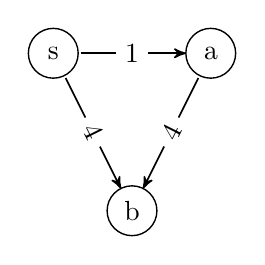
\begin{tikzpicture}[scale = 1.0, transform shape]
    \Vertex[x=0,y=2]{s}
    \Vertex[x=2,y=2]{a}
    \Vertex[x=1,y=0]{b}
    \tikzstyle{LabelStyle}=[fill=white,sloped]
    \tikzstyle{EdgeStyle}=[post]
    \Edge[label=$1$](s)(a)
    \Edge[label=$4$](s)(b)
    \Edge[label=$4$](a)(b)
\end{tikzpicture}\\
\\
es ist ersichtlich, dass der kuerzeste Weg aus $G$ von s ueber a nach b mit den Kanten $K = \{(s,a),(a,b)\}$ verlaueft.\\
Wuerde man nun aber den Dijkstra-Algorithmus auf $G'$ anwenden waere die kuerzeste Verbindung von s nach b mit den 
Kanten $K' = \{(s,b)\}$. Es gilt $K \neq K'$ damit ist Bobs Verfahren nicht Korrekt.\\

\subsubsection \
Bellman-Ford Algorithmus:\\
$d_i$ steht je fuer den i-ten durchlauf.\\
\begin{tabular}{l|l|l|l|l}
\end{tabular}
\\
Negative Zyklen:\\
\end{document}\\
